
\section{Dominio cerrado (Popescu/World)}
\subsection{Introducción}
\begin{frame}
\frametitle{Introducción}
\begin{itemize}
  \item Sistema que implementa el modelo propuesto por Popescu en [Popescu et al. 2003a] y  [Popescu et al. 2003b].
  \item Define concepto de tratabilidad semántica y traduce preguntas semánticamente tratables en consultas SQL
  \item Código implementado en java, accesible en http://github.com/julian3833/popescu-world
  \item Testeado sobre base de datos relacional de juguete provista por MySQL, llamada World, con información geográfica básica de países, ciudades e idiomas.
  \item Sistema de funcionalidad acotada con soporte solo para el inglés.
\end{itemize}
\end{frame}

\subsection{Modelo teórico}

\begin{frame}
  \frametitle{Dominio de problemas}
   \begin{block}{Dominio acotado y específico}<1->
      \begin{itemize}
          \item Restaurants, bancos, vuelos, libros, etcétera (pero solo uno)
          \item Bases de datos relacionales $\rightarrow$ datos estructurados
          \item Question answering como interfaz para una base de datos
          \item Traducir pregunta a SQL
      \end{itemize}
    \end{block}
\end{frame}

\begin{frame}
  \frametitle{Ejemplo}
  \begin{block}{Pregunta}<2->
      When did Albert Einstein die?
  \end{block}
  \begin{columns}<3->
      \begin{column}{.5\textwidth}
      \end{column}
      \begin{column}{.1\textwidth}
      \begin{tikzpicture}[>=stealth, rotate border/.style={shape border uses incircle, shape border rotate=270}]
              \node[rotate border=-40, fill=black, minimum height=1.0cm, single arrow, single arrow head extend=.3cm, single arrow head indent=.1cm, inner sep=1.5pt] (arrow) {};
          \end{tikzpicture}
      \end{column}
      \begin{column}{.3\textwidth}
          %Question Answering
      \end{column}
      \begin{column}{.5\textwidth}

      \end{column}
  \end{columns}

  \begin{exampleblock}{Consulta SQL}<3->
      \textbf{SELECT} death\_date \textbf{FROM} scientists

      \textbf{WHERE} name $=$ `Albert Einstein'
  \end{exampleblock}
  \begin{columns}<4->
      \begin{column}{.5\textwidth}
      \end{column}
      \begin{column}{.1\textwidth}
      \begin{tikzpicture}[>=stealth, rotate border/.style={shape border uses incircle, shape border rotate=270}]
              \node[rotate border=-40, fill=black, minimum height=1.0cm, single arrow, single arrow head extend=.3cm, single arrow head indent=.1cm, inner sep=1.5pt] (arrow) {};
          \end{tikzpicture}
      \end{column}
      \begin{column}{.3\textwidth}
          %Question Answering
      \end{column}
      \begin{column}{.5\textwidth}

      \end{column}
  \end{columns}

  \begin{alertblock}{Respuesta}<4->
      April 18th, 1955
  \end{alertblock}

\end{frame}


\begin{frame}
  \frametitle{Modelo teórico}
      \begin{itemize}
          \item Popescu et al. $\rightarrow$ QADB, Precise
          \item Tratabilidad semántica de una pregunta $q$ en el contexto de una DB $d$.
          \item Las preguntas no tratables se rechazan, las tratables se traducen.
          \item Motivación: no se puede fallar activamente (mal interpretar)
      \end{itemize}
\end{frame}





\begin{frame}
  \frametitle{Tratabilidad semántica / motivación}
      \begin{itemize}
          \item La complejidad de las preguntas en lenguaje natural es arbitrariamente grande.
          \item Las preguntas semánticamente tratables son preguntas fáciles pero abarcativas
          \item Distinguir un subconjunto 1) \textit{tratable} y 2) \textit{abarcador}
          \item Rechazar y pedir reformulación de las no tratables
          \begin{itemize}
            \item Es mejor no dar respuesta a dar una mala. Conservar la confianza en el sistema.
          \end{itemize}
      \end{itemize}
\end{frame}

\begin{frame}
  \frametitle{Tratabilidad semántica / idea coloquial}
    \begin{block}{Tratabilidad semántica en el contexto de una DB}<1->
      \begin{itemize}
          \item Una Q-word (Qué, quién, cuándo, dónde, etc.)
          \item Pares de atributos y valores
          \item Valores sueltos
          \item Términos no significativos y menciones a relaciones
          \item Por ejemplo:
            \begin{itemize}
              \item ¿{\color{green}Qué} {\color{orange}bancos} de la {\color{red}empresa Credicoop} están localizados en el {\color{blue}barrio} de {\color{blue}Coghlan}?
              \item ¿{\color{green}Quién} era el {\color{red}presidente} de {\color{red}México} en {\color{orange}1993}?
            \end{itemize}
      \end{itemize}
    \end{block}
\end{frame}

\fontsize{9.5pt}{7.2}\selectfont
\begin{frame}
  \frametitle{Definiciones (1): Elemento, qword, compatibilidad, token, marcador sintáctico}
   \begin{itemize}
      \item Elementos de una DB: Relaciones, Atributos y Valores
      \item Qwords - pronombres interrogativos
      \begin{itemize}
          \item \{What, where, which, when, who\}
          \item \{Qué, dónde, cuál, cuándo, quién\}
      \end{itemize}
      \item Compatibilidad 
      \begin{itemize}
          \item Valor con sus atributo
          \item Atributos con sus relaciones
          \item Valor con las relaciones de sus atributos
          \item Q-words compatibles con atributoes
          \begin{itemize}
            \item Definición a mano especifica por DB
          \end{itemize}
      \end{itemize}
      \item Token: un conjunto de lemas de palabras de la pregunta que corresponden a un elemento de la base de datos.
      \begin{itemize}
            \item Por ejemplo, \{experiencia, requerir\} y \{experiencia, necesario\} son dos tokens para ``Experiencia Requerida''
      \end{itemize}
      \item Marcador sintáctico: palabras que no aportan a la interpretación de la pregunta, definidas a mano
    \end{itemize}
\end{frame}

\fontsize{9.5pt}{7.2}\selectfont
\begin{frame}
  \frametitle{Definiciones (2): Correspondencia entre tokens y elementos}
  \begin{itemize}
    \item Cada elemento de la base de datos se separa en palabras individuales:
    \begin{itemize}\fontsize{9.5pt}{7.2}\selectfont
      \item “Experiencia Requerida” $\rightarrow$ \{Experiencia, Requerida\}
    \end{itemize}
    \item Se genera un conjunto de sinónimos para cada palabra usando Wordnet:
    \begin{itemize}\fontsize{9.5pt}{7.2}\selectfont
      \item experiencia $\rightarrow$ \{experiencia, conocimiento, habilidad,...\}
      \item requerida $\rightarrow$ \{requerida, necesaria, indispensable,...\}
    \end{itemize}
    \item Se toman los lemas o raíces de todas las palabras
      \begin{itemize}\fontsize{9.5pt}{7.2}\selectfont
        \item experiencia $\rightarrow$ \{experiencia, conocimiento, habilidad,...\}
        \item requerida $\rightarrow$ \{requerir, necesario, indispensable,...\}
    \end{itemize}
    \item Se generan tokens combinando los lemas de los sinónimos de cada elemento:
    \begin{itemize}\fontsize{9.5pt}{7.2}\selectfont
        \item tokens = \{(experiencia, requerir), (conocimiento, requerir), (habilidad, requerir),(experiencia, necesario), (conocimiento, necesario), (habilidad, necesario),(experiencia, indispensable), (conocimiento, indispensable), (habilidad, indispensable)\}
    \end{itemize}
    \item Este conjunto de tokens son los tokens que se corresponden con el elemento
    \item Un token tiene tipos dependiendo a qué elementos corresponda
  \end{itemize}
\end{frame}

\begin{frame}
\frametitle{Definiciones (3): tokenización completa, asociación sintáctica}

  \begin{itemize}
    \item \textbf{Tokenización completa de una pregunta \textit{q}}:  cualquier conjunto de tokens en los que cada término que no es un marcador sintáctico de $q$ aparece en exactamente un token del conjunto.
    \begin{itemize}
      \item Una partición de tokens (como fueron definidos) de la pregunta $q$
    \end{itemize} 
    \item \textbf{Asociación sintáctica}: dos tokens están sintácticamente asociados en $q$ si cumplen ciertas restricciones sintácticas.
    \begin{itemize}
      \item Modelado con una función $attachment($ t1, t2, q $) \rightarrow booleano$
    \end{itemize} 
   \end{itemize}
\end{frame}

\fontsize{9.5pt}{7.2}\selectfont
\begin{frame}[<+->]
\frametitle{Definiciones (4): traducción válida}
 Una \textbf{traducción válida} es un mapeo de una tokenización completa de $q$ en elementos de $E$ que cumple 3 condiciones:
\begin{enumerate}
  \item Cada token se corresponde con un único elemento de $E$.
  \item Cada token de atributo se relaciona con un único token de valor, cumpliendo que:
  \begin{itemize}
    \fontsize{9.5pt}{7.2}\selectfont
    \item el atributo de la base de datos que corresponde al token de atributo y el valor de la base de datos que corresponde al token de valor son compatibles
    \item ambos tokens están sintácticamente asociados
   \end{itemize}
  \item Cada token de relación está relacionado a un token de atributo o bien a un token de valor, cumpliendo las siguientes condiciones:

  \begin{itemize}
    \fontsize{9.5pt}{7.2}\selectfont
    \item la relación de la base de datos que corresponde al token de relación y el elemento de la base de datos que corresponde al token de atributo o token de valor son compatibles
    \item ambos tokens (token de relación - token de atributo o bien token de relación - token de valor) están sintácticamente asociados
  \end{itemize}
\end{enumerate}
\end{frame}

\fontsize{10pt}{11.2}\selectfont
\begin{frame}[<+->]
\frametitle{Definiciones (5): Semánticamente tratable}
Si una pregunta tiene solo una q-word y al menos una traducción válida entonces es \textbf{semánticamente tratable}

\bigskip
\bigskip

Y cada traducción válida de $q$ determina una posible consulta SQL:
\bigskip
\centering
\begin{tabular}{ r | l }
SELECT &  Elementos apareados con qwords \\
WHERE & Pares de atributos y valores generados por el Matcher\\
FROM & Todas las relaciones mencionadas \\
\end{tabular}
\end{frame}


\fontsize{9.5pt}{7.2}\selectfont
\begin{frame}
\frametitle{Precise}

  \begin{block}{El sistema utilizado por Popescu et al.}<1->
      \begin{itemize}
          \item Dada una pregunta $q$, determina si es semánticamente tratable y si lo es, genera una consulta SQL correspondiente. Si no, la rechaza pidiendo una reformulación.
        \end{itemize}
    \end{block}
   \begin{block}{Lexicon}<1->
      \begin{itemize}
          \item Sinónimos lematizados de todas las relaciones, atributos y valores
          \begin{itemize}
            \item Wordnet
          \end{itemize}
          \item Determina qué términos son comprensibles de una pregunta
          \item Las preguntas tratables tienen solamente marcadores sintácticos + palabras del lexicon.
        \end{itemize}
    \end{block}
    \begin{block}{Matcher}<1->
      \begin{itemize}
          \item La pieza clave.
          \item Relaciona cada valor con un único atributo, implícito o explícito usando un algoritmo de max flow.
      \end{itemize}
    \end{block}
\end{frame}

\fontsize{9.5pt}{7.2}\selectfont
\begin{frame}
\frametitle{Precise / módulos}

\begin{itemize}
  \item Lexicon: encargado de generar, para cada elemento de la base de datos, el conjunto de tokens sinónimos que se utilizará para verificar correspondencia.
  \item Tokenizer: encargado de generar todas las tokenizaciones completas de la pregunta y, para cada token, consultar al lexicon y retornar la lista de elementos de la base de datos que le corresponden.
  \item Matcher: encargado de verificar que las tokenizaciones completas y los elementos correspondientes generados por el tokenizer cumplan las condiciones 1 a 3 utilizando el modelo de grafos y el algoritmo max-flow recién ilustrado.
  \item Parser plug-in: el módulo computa la función de asociación sintáctica, basándose en el parse tree de Charniak.
  \item Query generator: dado el conjunto de elementos de la base de datos traducido de la pregunta, genera una query SQL.
  \item Equivalence Checker: verifica si diferentes queries son la misma formulada de diferentes maneras.
\end{itemize}
\end{frame}


\fontsize{11pt}{7.2}\selectfont
\begin{frame}
\frametitle{Ejemplo}
\begin{figure}
  \centering
    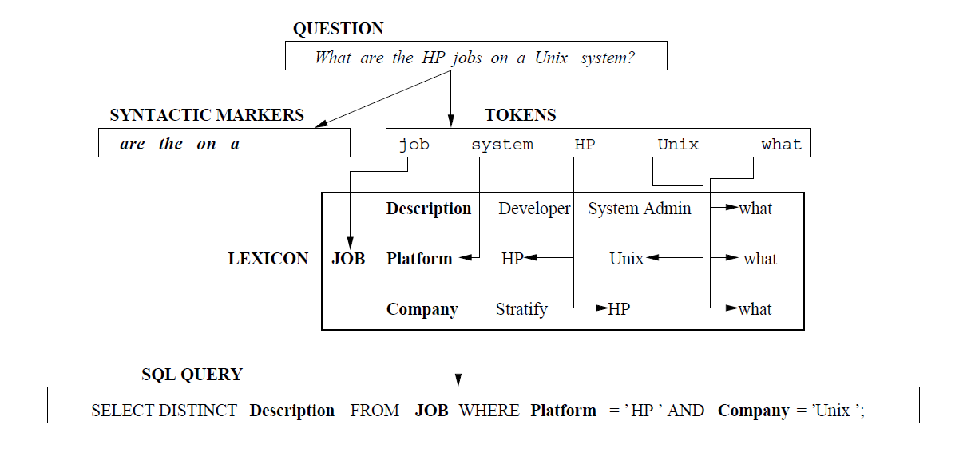
\includegraphics[scale=.7]{graficos/popescu-example}
  \caption{La traducción de la pregunta ``What are the HP jobs on a Unix system?'' a una consulta SQL}
  \label{fig:popescu-example}
\end{figure}

\end{frame}


\begin{frame}

\frametitle{Ejemplo}

\begin{figure}
  \centering
    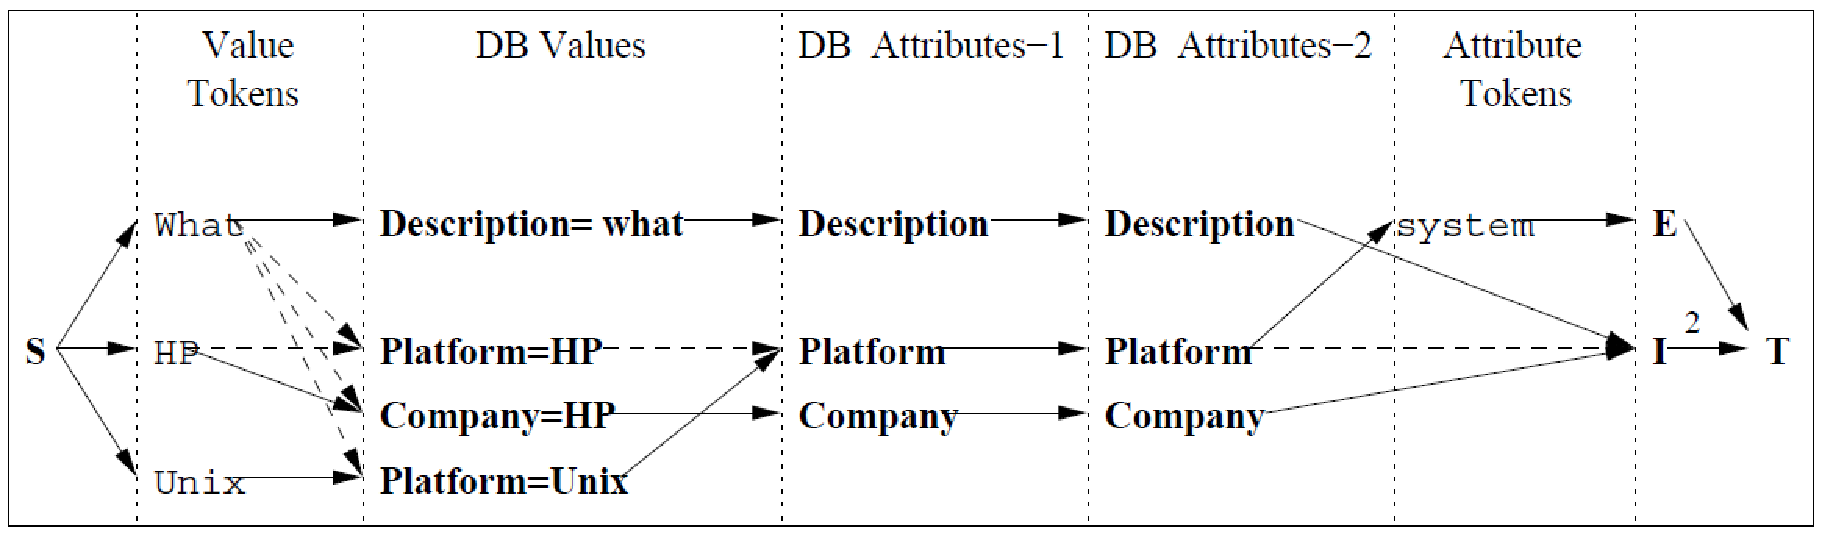
\includegraphics[scale=0.3]{graficos/popescu-example-2}
  \caption{El grafo de atributos y valores creado por Precise para la pregunta ``What are the HP jobs on a Unix system?''}
  \label{fig:popescu-example-2}
\end{figure}
\end{frame}

\subsection{Implementación}
\subsubsection*{Base de datos}
\begin{frame}
\frametitle{Base de datos: World (Country, City y CountryLanguage)}
\begin{figure}
    %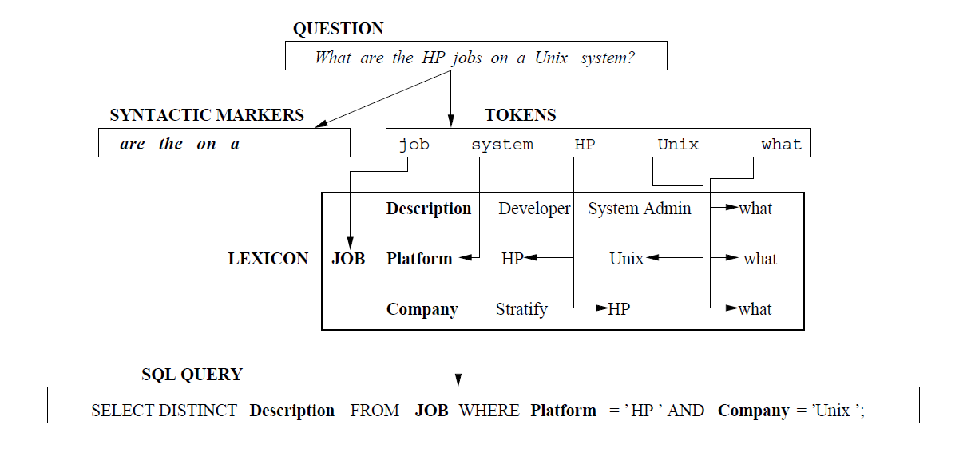
\includegraphics[scale=1.0]{graficos/popescu-example}
    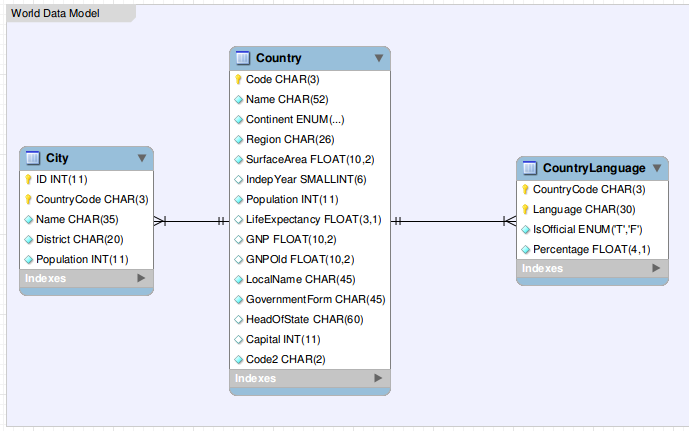
\includegraphics[width=9.823cm,height=6.004cm]{graficos/fuentes/world-db.png}
\end{figure}

\end{frame}
\subsubsection*{Implementación}
\begin{frame}
\frametitle{Lexicón}
  El lexicón es el módulo encargado de generar un conjunto de tokens para cada elemento de la base de datos. Una vez construido este conjunto, las responsabilidades del módulo son las siguientes:
\begin{itemize}
  \item Dado un lema, devolver el conjunto de tokens que lo contienen ($getTokens()$).
  \item Dado un token, devolver el conjunto de elementos de la base de datos que le \textit{corresponden} ($getMatchingElements()$).
  \item Wordnet. TokenAugmenter. Polisemia.
\end{itemize}
\end{frame}

\begin{frame}
\frametitle{TokenAugmenter}
\begin{center}
\begin{table}[h]
\centering
\begin{tabular}{| l |  p{8cm} |}
\hline
Elemento original & Sinónimos \\ \hline
head of state & president, leader, emperor, king \\ \hline
region & location\\ \hline
surface area & size, total size, square kilometers, km2\\ \hline
independence year & independent, independency\\ \hline
\end{tabular}
\caption{Sinónimos introducidos por el Token Augmenter}
\label{table:token-augmenter}
\end{table}
\end{center}
\end{frame}


\begin{frame}
\frametitle{Compatibilidad de Qwords}
\begin{center}
\begin{table}[h]
\centering
\begin{tabular}{| l |  p{8cm} |}
\hline
Qword & Atributos relacionados \\ \hline
What & \textbf{Name}, District, Population, Code, Continent, SurfaceArea, LifeExpectancy, GNP, LocalName, GovernmentForm,
                         Capital, IsOfficial, Percentage, Region \\ \hline
Which & Los mismos que para what\\ \hline
Where & \textbf{Region}, Continent, Capital, District\\ \hline
Who & \textbf{HeadOfState}\\ \hline
When & \textbf{IndependenceYear}\\ \hline
\end{tabular}
\caption{Atributos compatibles con cada Qword}
\label{table:atributos-qwords}
\end{table}
\end{center}

\end{frame}

\fontsize{9.5pt}{7.2}\selectfont
\begin{frame}
\frametitle{Tokenizer}
\begin{enumerate}
\item Separar la pregunta en palabras, eliminar puntuaciones y pasar a lower case.
\item Lematizar las palabras. Para esto usamos Freeling
\item Eliminar marcadores sintácticos.
\item Para cada lema, obtener todos los tokens que lo contienen del Lexicon (método getTokens).
\item Para cada token potencial (resultado del paso anterior) verificar que todos sus lemas estén presentes en el conjunto de lemas de la pregunta original.
\item Generar el conjunto de partes de todos los tokens hasta aquí obtenidos.
  Probando con cada elemento del conjunto de partes en lugar de utilizar solamente el conjunto original podemos obtener subconjuntos que cumplan también la condiciones requeridas para considerarse una tokenización completa (evaluados en 7).
\item Para cada uno de estos subconjuntos, verificar 1) que sus tokens cubran completamente los lemas significativos de la pregunta original y 2) que no haya lemas repetidos entre los tokens.
\end{enumerate}
\end{frame}

\begin{frame}
\frametitle{Matcher}
  \begin{itemize}
    \item {\color{red} FILL ME}
  \end{itemize}
\end{frame}

\begin{frame}
\frametitle{MappingFilter, QueryGenerator, MainProcessor}
  \begin{itemize}
    \item {\color{red} FILL ME}
  \end{itemize}
\end{frame}
\subsubsection*{Ejemplos}
\begin{frame}
\frametitle{Ejemplos}
  \begin{itemize}
    \item {\color{red} FILL ME}
    \item Who is the head of state of Zimbabwe?
    \item What caribbean countries are also considered north american?
  \end{itemize}
\end{frame}
\subsubsection*{Conclusiones y limitaciones}
\begin{frame}
\frametitle{Conclusiones y limitaciones}
  \begin{itemize}
    \item {\color{red} FILL ME}
  \end{itemize}
\end{frame}
